\documentclass[tikz,border=5pt]{standalone}
\usepackage{pgfplots}
\pgfplotsset{compat=1.18}

\definecolor{corba}{HTML}{365FB3}
\definecolor{assimptota}{HTML}{C2415D}

\begin{document}
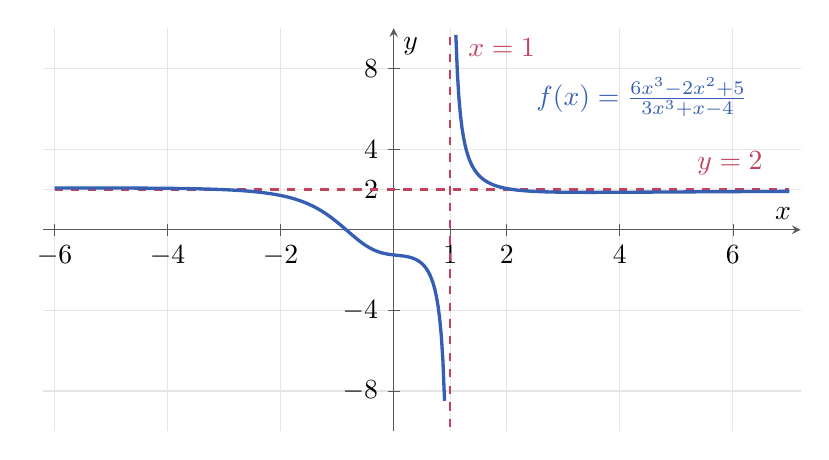
\begin{tikzpicture}
  \begin{axis}[
    width=11.2cm,
    height=6.7cm,
    axis lines=middle,
    xmin=-6.2,
    xmax=7.2,
    ymin=-10,
    ymax=10,
    xlabel={$x$},
    ylabel={$y$},
    xtick={-6,-4,-2,1,2,4,6},
    ytick={-8,-4,2,4,8},
    axis line style={black!65},
    tick style={black!65},
    grid=major,
    grid style={black!10},
    clip=false,
  ]
    \addplot[assimptota, dashed, thick] coordinates {(1,-9.8) (1,9.8)};
    \addplot[assimptota, dashed, thick, domain=-6:7] {2};

    \addplot[corba, very thick, domain=-6:0.9, samples=240]
      {(6*x^3-2*x^2+5)/(3*x^3+x-4)};
    \addplot[corba, very thick, domain=1.1:7, samples=220]
      {(6*x^3-2*x^2+5)/(3*x^3+x-4)};

    \node[anchor=south west, text=assimptota]
      at (axis cs:1.15,8.1) {$x=1$};
    \node[anchor=south east, text=assimptota]
      at (axis cs:6.7,2.25) {$y=2$};
    \node[anchor=south west, text=corba]
      at (axis cs:2.35,5.1) {$f(x)=\frac{6x^3-2x^2+5}{3x^3+x-4}$};
  \end{axis}
\end{tikzpicture}
\end{document}
